\documentclass{article}
\usepackage[utf8]{inputenc}
\usepackage{amsmath}
\usepackage{graphicx} %for images
\usepackage[utf8]{inputenc} %for ToC
\usepackage{lscape}%for landscape layout
\usepackage{rotating}%to rotate figs
\usepackage{geometry}%to change margins
\usepackage{hyperref} %for links
\hypersetup{
linktoc=all,  
    colorlinks,
    citecolor=black,
    filecolor=black,
    linkcolor=black,
    urlcolor=black
}

%for bibliography"
%with biblatex
%\usepackage[style=authoryear]{biblatex}
%\addbibresource{references.bib}
% or with natbib
\usepackage{natbib} 
\usepackage{har2nat}
%\bibliography{references.bib}

\renewenvironment{abstract}
 {\normalsize
  \begin{center}
  \bfseries \large \abstractname \vspace{-.5em}\vspace{0pt}
  \end{center}
  \list{}{
    \setlength{\leftmargin}{.5cm}%
    \setlength{\rightmargin}{\leftmargin}%
  }%
  \item\relax}
 {\endlist}

\begin{document}
\pagenumbering{roman}
\begin{titlepage}
    \begin{center}
          
        
        \LARGE
        Progression paper  
        \vspace{4cm}
        
        \Huge
        \textbf{Understanding how pharmaceutical pollutants move through river catchments}
            
        \vspace{1cm}
        
        \LARGE    
        \textbf{Julia Costescu} 
        $^1^,^2\\
        
        \vspace{1cm}
        
        \normalsize
        \textbf{         Supervised by}\\
        
         Prof. Louise Bracken$^1^,^2$,\\
            Dr. Laura Turnbull-Lloyd$^1^,^2$ \\
            and Damian Crilly$^3$\\
        
        
        \vspace{1cm}
            
        
\includegraphics[height=2cm]{logo.png}
            
        \Large
        Geography Department$^1$\\
        i-CONN Network$^2$\\
        Environment Agency$^3$\\
        \vspace{1cm}
        March 2021
            
    \end{center}

%\clearpage
%\title{Progression paper}
%\title{Understanding how pharmaceutical pollutants move through river catchments}
%\author{Julia Costescu}
%\date{February 2021}

\end{titlepage}

\begin{abstract} \addcontentsline{toc}{section}{Abstract}
The blah blah blah (To be continued...)
\end{abstract}

\clearpage
\tableofcontents



\clearpage
\pagenumbering{arabic}
\section{Introduction}
%Example superscript:
Enabled by recent developments in analytical methods \citep{Knoll2020TrendsSamples}, screening studies point to the near ubiquitous presence of pharmaceuticals in surface waters across the world \citep{Bai2018OccurrenceWatersheds,Hughes2013GlobalSystems,Kolpin2002PharmaceuticalsReconnaissance}. These findings, together with a growing body of evidence of negative environmental impacts, have turned the presence of pharmaceuticals in the environment into an issue of growing interest and concern, especially considering the expected increase in the use of medication on a global scale \citep{Hughes2013GlobalSystems,UNEP2017PharmaceuticalsIssue}. 

After consumption by humans, or animals in the case of veterinary pharmaceuticals, a high proportion of the mass of applied pharmaceuticals (or their metabolites), sometimes more than 70\% \citep{Pal2010ImpactsEffects}, is excreted and released into the environment. This release is either direct, in the case of animal manure, septic tank seepage or through sewage storm overflow, or indirect, after incomplete removal by wastewater treatment plants (WWTPs) \citep{Yao2018OccurrenceStudy}. In fact, WWTP effluent represents the main pathway for pharmaceuticals to reach water courses \citep{Daughton2001PharmaceuticalsOverview}, among several others (see Figure \ref{fig_sources}). The constant consumption and subsequent discharge into aquatic ecosystems of many pharmaceuticals through these pathways causes their presence in environmental waters to be considered to be pseudo-permanent, regardless of their half-lives \citep{Feng2018Metal-mediatedAssessment}.

Pharmaceutically active compounds are often found only in trace amounts in surface waters \citep{Quesada2019SurfaceReview}. However, a growing body of evidence shows that these concentrations are sufficient to cause significant harm to non-target aquatic organisms and ecosystems \citep{Brodin2014EcologicalAlterations,Miller2018AFauna,Shaliutina-Kolesova2020TheReview}. This conclusion is supported by ecotoxicological studies performed at the laboratory, field and ecosystem scale \citep{ausderBeek2016PharmaceuticalsPerspectives}. Notably, invertebrates are affected (daphnids and water fleas in particular \citep{Pal2010ImpactsEffects}), but so are algae and vertebrates, such as amphibians and fish. Impacts may be expressed in terms of morbidity and mortality \citep{Kummerer2009TheChallenges} of standard laboratory organisms, but there are also less obvious but equally harmful endpoints \citep{Daughton2001PharmaceuticalsOverview}: neurobehavioral \citep{Brodin2014EcologicalAlterations,Shaliutina-Kolesova2020TheReview}, immunological, and endocrine homeostasis alterations (for example, by causing an increased incidence of intersex characteristics in fish \citep{Dong2015FateStream}). A further cause for concern has been the documented exposure to pharmaceuticals in vulnerable protected areas \citep{Bradley2020ExposureRegion}. Finally, the persistent presence of antibiotics in the environment coupled with their interactions with microbiota has been shown to cause a rise in antibiotic resistant pathogens \citep{Leonard2018ExposureSurvey,Segura2009ReviewWaters}.

As for the eventual fate of pharmaceuticals, during in-stream transport, they undergo natural attenuation, primarily through sorption and biodegradation, but also photodegradation and hydrolysis \citep{Dong2015FateStream}. However, these transformations often do not bring contamination levels down below predicted no-effect concentrations (PNEC) \citep{Li2014OccurrenceSoil}, in which case engineering solutions may be used to remove pharmaceuticals and their metabolites. However, removal rates in conventional WWTPs vary significantly among the different compounds, from 100\% for the antibacterial compound sulfamethazine to just 3\% for erythromycin, an antibiotic, in a review by \citet{Verlicchi2012OccurrenceReview}. Thus, many studies conclude that there is a need for tertiary treatment, such as are ultra- and nano-filtration, adsorption \citep{Quesada2019SurfaceReview}, advanced oxidation \citep{Feng2018Metal-mediatedAssessment}, and reverse osmosis. Bioremediation has also been shown to aid with degradation or removal of certain compounds through the actions of microbes, plants \citep{Li2020PhytoremediationCycle} and animals which control biotic and abiotic factors in order to promote the transformation or immobilization of the target contaminants \citep{Gavrilescu2015EmergingBioremediation,Patel2020EmergingReview}.
    
While the issue of Pharmaceuticals in the Environment (PiE) has seen a rapid increase in interest, under-studied geographic regions and research gaps remain. Most pressingly, there is a limited understanding of how pharmaceuticals are transported throughout river catchments as well as of their spatial and temporal distribution. This understanding is essential in order to inform risk assessment efforts and design targeted monitoring and mitigation practices with optimized intervention points in terms of available resources and associated carbon costs \citep{Domercq2018EmissionResolution}. To this end, higher sampling resolution is called for, in both spatial and temporal resolution, which is required in order to understand transport times through the watercourse, seasonality or longer-term trends in pharmaceutical loading \citep{Burns2018TemporalSystem}. Furthermore, there have been few attempts of a truly quantitative assessment of the relative contributions of the different sources and pathways for pharmaceutical pollution \citep{Comoretto2005ComparingRiver,Kookana2014PotentialCountries}, and we are only beginning to understand the multitude of factors, such as land use or demographic structure, that affect the composition and level of pharmaceutical contamination in environmental waters. In the UK, PiE research has started more recently \citep{Ashton2004InvestigatingKingdom,Bound2006PredictedAssessment} and has mainly been clustered around south-east England and south Wales \citep{Kay2017WidespreadWaters}.

The proposed research sets out to build a framework using both available monitoring data and field data to describe the state of pharmaceuticals in the environment in the North East region and subsequently construct a system model to assess connectivity between elements of the catchment system and optimal intervention points. 


%See figure \ref{fig_Sources} on page \pageref{fig_Sources}.
\clearpage
\section{Theoretical Framework}
Pharmaceuticals are generally defined as substances used to diagnose, treat, or prevent diseases in humans or animals, including recreational and illicit drugs \citep{Quesada2019SurfaceReview}. They are part of what are known as emerging contaminants, a group which also includes pesticides, surfactants, flame retardants, personal care products and others \citep{ausderBeek2016PharmaceuticalsPerspectives,Vargas-Berrones2020Emerging-Nonylphenol-}. Another term used for this group is micro-pollutants, so called because their concentration in the aquatic environment is in the order of µg/L to ng/L \citep{Kummerer2009TheChallenges}.  
Pharmaceuticals possess a series of distinguishing properties. They are resistant to biodegradation by design, so as to achieve their medical purposes; however, this is also a cause for their persistence in the environment \citep{Fatta-Kassinos2011PharmaceuticalResearch}. Their physico-chemical characteristics, such as pH-dependent solubility and polarity, have an impact on their environmental fate \citep{Kummerer2009TheChallenges}. As highly polar molecules, pharmaceutical compounds are less likely to be efficiently removed by standard WWTPs \citep{Mompelat2009OccurrenceWater}. Likewise, pharmaceuticals are lipophilic which enables passage through membranes and poses an increased risk to exposed organisms \citep{UNEP2017PharmaceuticalsIssue}. Pharmaceuticals are intended to undergo metabolic reactions in the body of target organisms that can lead to the formation of metabolites - compounds with different structure and properties which may pose their own risks to the environment \citep{Quesada2019SurfaceReview}.  

The multifaceted field of PiE remains a relatively new field, having been established in earnest barely two decades ago \citep{Daughton2016PharmaceuticalsAnalysis}. In order to approach the issue of PiE from a holistic perspective, the proposed research is situated at the nexus of three intersecting frameworks – the Source-Pathway-Receptor model (SPR), Integrated Catchment Management (ICM) and the field of Connectivity Science (CS)  (Figure \ref{fig_framework}). 

\begin{figure}[h]
    \centering
    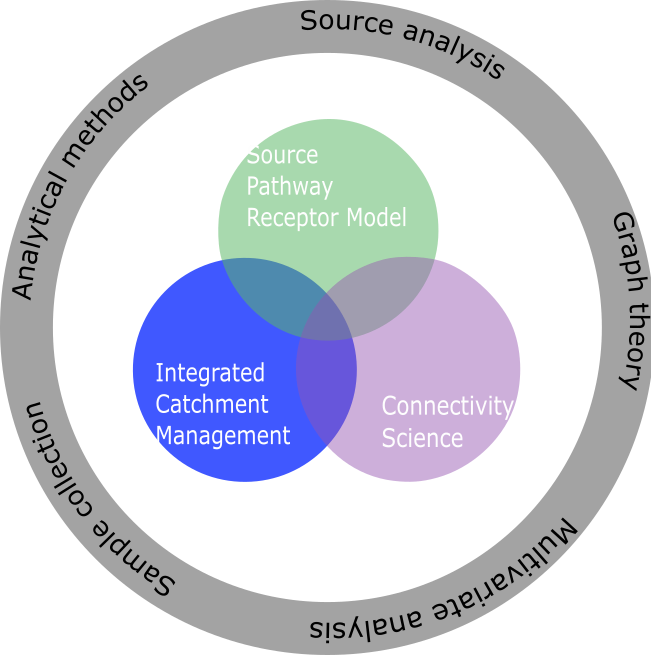
\includegraphics[height=8cm]{fig_framework.png}
    \caption{Theoretical framework circumscribing the proposed research.}
    \label{fig_framework}
\end{figure}

The SPR is a conceptual model which describes the flow of contaminants from each source, through transport pathways  and to the eventual receptors, which, depending on the scale of interest, may be environmental compartments or organisms or even at sub-organism scale \citep{Holdgate1979APollution.}. In systems as complex as river catchments, SPR acts as a system model, providing a more comprehensive understanding of underlying processes and mechanisms before further quantitative analyses \citep{Narayan2012SystemConcept,Waldschlager2020Thereview}. 

ICM was introduced as an adaptive planning and action process that recognizes the catchment as the natural scale for managing ecosystem processes \citep{Fenemor2011IntegratedKnowledge}. Defining the catchment as the fundamental unit naturally reflects the multitude of environmental processes and human activities that influence risk levels and the understanding of which is essential for efficient and sustainable management. ICM emphasizes the need for interdisciplinarity and knowledge integration \citep{Voulvoulis2012WaterApproach}, sometimes referred to as horizontal integration, as well as participation, or vertical integration, between the relevant experts, policy and the public \citep{Rollason2018EvaluatingManagement}. 

Lastly, an approach that may help address the research needs identified in the field of pharmaceutical contamination is that of network science, which aims to conceptualize complex systems such as river networks and analyze their behavior as a result of the interactions between their constituent parts \citep{Bullmore2009ComplexSystems}. This framework often employs graph theory as a useful mathematical tool to describe such systems and solve network-related problems \citep{Anderson2020ComplexApplications,Phillips2015GraphGeosciences}. 

These three branches are naturally aligned as they all take a systems approach to exploring fluxes of water, nutrients and sediment through the landscape, but each brings a new set of tools and conceptual models for understanding and tackling existing problems in this field. While SPR offers an understanding of the physical components involved in the flow of contaminants at any scale, ICM provides the fundamental unit as well as the management perspectives required to define and address such environmental challenges. Finally, connectivity science represents a quantitative framework that can offer informed decision support for policy makers.

\subsection{The Source-Pathway-Receptor Model}
In the case of PiE, an SPR model adapted from \citep{Stuart2012ReviewGroundwater} is represented in Figure \ref{fig_framework} and explored in more detail in Table \ref{table_sources} . The main pathway for entry into surface waters is widely considered to be through WWTP effluent, which itself owes most of its pharmaceutical load to domestic use and excretion \citep{Larsson2007EffluentPharmaceuticals}, discharged in what are essentially point sources of pollution. Improper disposal (flushing of unused medication) has also been signalled as being a significant issue, especially since it can be most easily addressed through awareness campaigns, although the relative contribution to contaminant loads may not be great \citep{Vatovec2016InvestigatingSetting}. Hospitals, industrial and animal farming activities also contribute to the load of WWTP effluent through their wastewater. Conversely, there are a number of non-point or diffuse sources, notably runoff from agricultural areas fertilized with the field application of sewage sludge containing compounds removed from WWTP influent or manure containing veterinary pharmaceuticals (as well as excrement deposited directly by livestock). A second diffuse pathway is that of septic tank leaching in areas detached from sewage infrastructure \citep{Comber2018ActiveConcern,Kookana2014PotentialCountries}.

\begin{figure}[t]
    \centering
    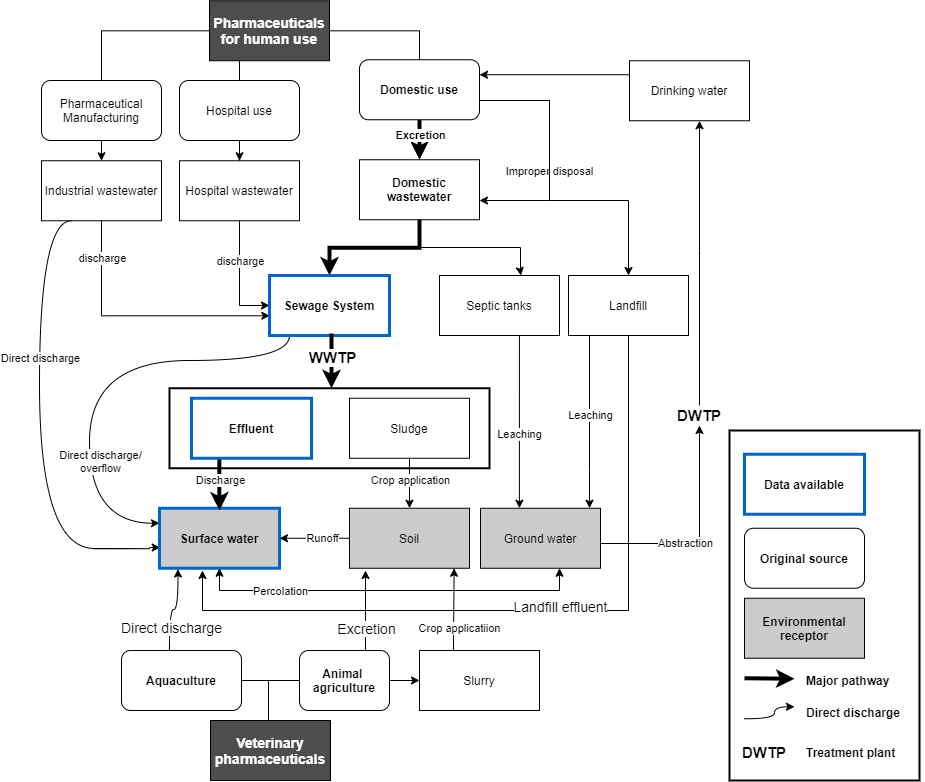
\includegraphics[height=10cm]{fig_sources.png}
    \caption{Sources of pharmaceuticals and pathways into the environment, adapted from Stuart et al. (2012).}
    \label{fig_sources}
\end{figure}

Due to data availability, this proposed research relies primarily on WWTP effluent as a main pathway for entering surface waters. However, an analysis of predictive factors and catchment-specific knowledge is intended to provide insight into other likely sources (see Section \ref{source_analysis}). For instance, septic tank distribution, inferred based on sewage infrastructure maps, or runoff contribution, estimated based on land use information, can be incorporated in constructing the catchment-level system.

In the  seminal work by \citet{Holdgate1979APollution.}, pathways were described within the environment, but the author also proposed diagrams exploring pathways within trophic chains or even within target organisms. Bioaccumulation is known to be a major factor in the fate of many environmental contaminants (Vargas-Berrones et al., 2020; Zenker et al., 2014), although there are indications from applications in aquaculture that in the case of pharmaceuticals, this may not constitute a large fraction of the environmental loading \citep{Rico2013ProbabilisticAsia}. Nevertheless, it would represent a valuable area of future research  \citep{Stuart2012ReviewGroundwater}, which has yet not been included in the conceptual model as data on this topic is not as readily available or comprehensive. As the field of PiE research has developed in recent years, several studies have examined how different factors influence patterns in pharmaceutical loads \citep{Burns2018TemporalSystem,Vatovec2016InvestigatingSetting}, which is essential in interpreting field measurements from a SPR perspective. However, lack of data and research means that uncertainty remains around spatial patterns in the landscape. For instance land use is a significant factor, as veterinary and human medicines closely tie in with rural and urban areas, concentrations can also be influenced by demographic factors, most notably by population density, a metric often used to predict pharmaceutical exposure \citep{Brodin2014EcologicalAlterations}, and seasonality and factors influencing short-term variation in pharmaceutical concentrations have also been subject of increasing research interest \citep{Burns2018ApplicationPharmaceuticals}.

\begin{landscape}
\begin{table}
  \caption{Examples of studies investigating the contribution of various Sources and Pathways.}
  \label{table_sources}
  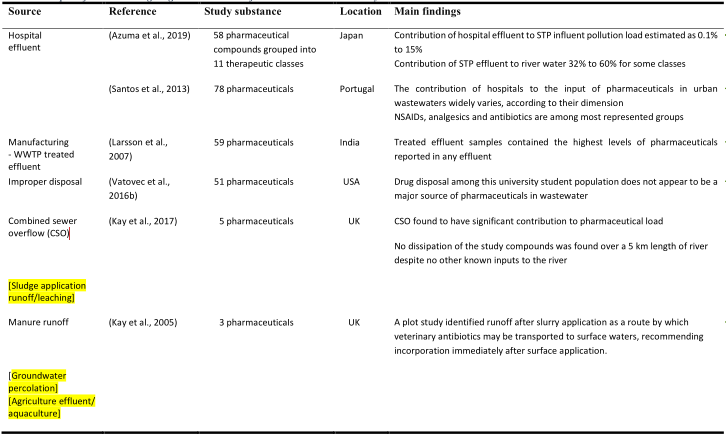
\includegraphics[width=\linewidth]{Table1.png}
\end{table}
\nocite{Santos2013ContributionPharmaceuticals,Azuma2019EnvironmentalJapan,Larsson2007EffluentPharmaceuticals,Vatovec2016InvestigatingSetting,Kay2017WidespreadWaters,Kay2005TransportLand}

%\begin{sidewaystable}[h!] % <--
  
 % \caption{Examples of studies investigating the contribution of various Sources and Pathways.}
 %  \label{tab:table1}
 % \begin{ruledtabular}
 % \begin{tabular}{lllll}
 % 	\toprule
 % 	\textbf{Source} & \textbf{Reference} & \textbf{Study substance} &
 % 	    \textbf{Location}&
 % 	    \textbf{Main findings}\\
 %   \midrule
 %   Hospital 
%effluent
% & \citep{Azuma2019EnvironmentalJapan} & 58 pharmaceutical compounds grouped into 11 therapeutic classes & Japan & Contribution of hospital effluent to STP influent pollution load estimated as 0.1% to 15%
%Contribution of STP effluent to river water 32% to 60% for some classes
%\\
%    2 & 10.1 & b\\
%    3 & 23.113231 & c\\
%    %\bottomrule
%  \end{tabular}
%  \end{ruledtabular}
  
%\end{sidewaystable}


\end{landscape}

\subsection{Integrated Catchment Management}
Prompted by the requirements of the Water Framework Directive (WFD) which prescribes an ‘integrated river basin management’ approach \citep{EuropeanCommission2000DIRECTIVEPolicy}, the onus in environmental management has in recent decades shifted towards a holistic and systemic view of sustainability. Consequently, governing bodies and agencies across the world as well as in the UK have adopted what is known as a ‘Catchment-Based Approach’\citep{Collins2010TrustingWales,DEFRA2013CatchmentEnvironment}. This paradigm considers the ecosystem in its entirety as opposed to the traditional focus on end-of-pipe measures and standard policies, and includes both land and water components and processes, as well as human-environment interactions \citep{Voulvoulis2016TheImplementation}. 

\subsection{Connectivity Science}
Graphs represent a set of nodes connected by links or edges that may be directed or undirected as well weighted or unweighted in order to describe the relation between the connected nodes. This relation may be in terms of strength of the interaction, topological distance, or cost (see an example in Figure \ref{fig_graph_schick}). Similarly to the use of the SPR model, using graph theory does not necessarily preclude the use of numeric models, instead it can often be used in tandem, with pollution or hydrologic models providing an input for determining edge weights for example. However, a graph theoretic approach has the advantage of providing a simple abstraction of intricate systems while having the flexibility of allowing different scenarios of change or intervention to be modeled and the resulting change in emergent properties to be assessed \citep{OHanley2005OptimizingBarriers}. In fact, graph theory emerged because of its algorithms for determining optimal solutions for problems such as the historic Seven Bridges of Königsberg problem \citep{Bullmore2009ComplexSystems}. Therefore, it can be a valuable decision-making tool for environmental management.

Because of their dendritic structure and role in the transport of sediment, water, and other environmental fluxes, river systems have been represented using graph-theoretical approaches in recent years in order to assess and manage issued emerging from anthropogenic activities \citep{Abed-Elmdoust2016ReorganizationApproach,Abed-Elmdoust2017EmergentApproach,Cieplak1998ModelsBasins,Eros2011NetworkApproach,Tejedor2015DeltaSurfaces}. A relevant application for the present research is the use of graphs in the study of impacts of river barriers (or conversely, dam removal) on fish mobility and population connectivity \citep{Sarker2019CriticalNetworks,Schick2007DirectedNetwork,Segurado2013PrioritizingApproach}. Studies in this area have been able to propose multi-objective approaches that provide priorities for barrier removal that take cost into consideration as well as maximizing accessible habitat gain for example \citep{OHanley2005OptimizingBarriers}. As opposed to the issue of pharmaceutical pollution, where fragmenting the contamination pathways would be the aim of environmental managers, in these studies the desired outcome would be restoring connectivity or preventing further fragmentation.

An emerging concept at the intersection of network science and graph theory is that of connectivity, which describes the degree of connectedness of system, in terms of either its structure or dynamic processes, which can give rise to emergent behavior \citep{Turnbull2018ConnectivityPerspective}. When applied within the field of hydrology, connectivity science has the potential to provide an integrated approach for the study of complex systems as called for within the framework of ICM  \citep{Lexartza-Artza2009HydrologicalImplications}. These approaches and their associated tools have the potential to provide a useful framework with which to examine patterns of pharmaceutical contamination within catchments and identify hotspots and effective intervention strategies.

In practical terms, connectivity is often analyzed through a number of indices calculated on the basis of the graph representation of the system \citep{Ali2010ShoppingCatchment,Heckmann2018IndicesLimitations}.  As an example, a similar graph-theoretical approach to provide a prioritization tool for dam removal proposed by \citet{Segurado2013PrioritizingApproach} computed the integral connectivity index (IIC) and assessed changes in its value for different dam removal scenarios.

\begin{figure}
    \centering
    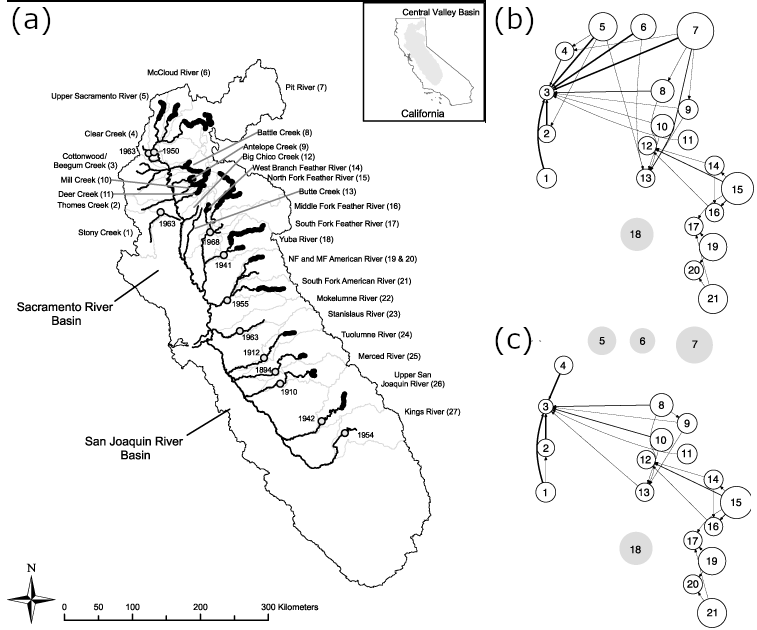
\includegraphics[height=10cm]{fig_graph_schick.png}
    \caption{An example of graph-theoretical representation of a river basin, taken from \citet{Schick2007DirectedNetwork}. The salmon populations present in numbered segments of the basin (a) are represented as nodes with directed and weighted edges (b) and (c). In this representation node size is proportional to habitat present in the respective watershed, and edge thickness corresponds the strength of population connectivity (percentage of receiving node population represented by individuals recruited from the originating node).(b) and (c) represent the network structure in two historical snapshots, with the addition of dams (c) causing changes in network structure and connectivity.}
    \label{fig_graph_schick}
\end{figure}

\clearpage
\section{Aim and Objectives}
\subsection{Aim}
The aim of this research is to improve our understanding of how pharmaceutical pollutants move through river catchments, in view of developing a network-based representation of their transport that will inform more tailored management practices, ultimately helping to determine more effective interventions to limit the impact of pharmaceutical pollutants on river ecosystems. 

\subsection{Objectives}
This aim will be addressed by meeting the following objectives:

\textbf{Objective 1 (O1): Developing an evidence base of sources and pathways for pharmaceuticals in UK river catchments. }\\
This objective entails compiling existing data sources and documenting the distribution of pharmaceuticals across the available sampling sites, as well as assessing the degree to which this data can be used to characterize the state of pharmaceutical pollution.

\vspace{5mm}
\textbf{Objective 2 (O2) : Exploring the controls on pharmaceuticals within UK catchments.}

In this step, the evidence base (O1) will be used to undertake exploratory analysis in order to understand:

\textbf{a) Seasonality:} variations in concentrations throughout the year may be caused by usage patterns, such as increased use of cold medication in winter months, or anti-allergy medication in spring \citep{Vatovec2016InvestigatingSetting}. Additionally, factors such as WWTP treatment efficiency (lower in winter months), and dilution due to variation in river discharge (higher in winter months) can also contribute to  seasonal patterns \citep{Comber2020SeasonalWaters}.

\textbf{b) Differences between urban and rural areas:} rural areas are expected to have higher prevalence of compounds found in veterinary medication, as well as receiving contaminants from an additional source in the form of runoff of sewage sludge used as fertilizer. Furthermore, the differences in sewage infrastructure – a higher proportion of households with septic tanks rather than connected to WWTPs in rural regions - might contribute to differences in the recorded pharmaceutical concentrations.

\textbf{c) Demographic controls:} specifically demographic factors, such as population density, age structure, deprivation, which may impact the types and quantities of pharmaceuticals used and detected in water samples.


\vspace{5mm}
\textbf{Objective 3 (O3): Determining the resolution of data required to adequately characterize the temporal dynamics of pharmaceuticals in rivers.}

By collecting field data at a higher spatial and temporal resolution on a local scale, a comparison with the existing data (O1) will be used to assess which resolution is sufficient to capture relevant spatial and temporal variation patterns.

\vspace{5mm}
\textbf{Objective 4 (O4): Determining the likely sources of pharmaceutical pollution from measured concentrations within a target catchment.}

This objective involves exploring the suitability of methods such as source analysis to solve the problem of tracing back likely sources within the catchment.

\vspace{5mm}
\textbf{Objective 5 (O5): Identifying points within the catchment where interventions for reducing pharmaceutical contamination would be most effective.}

Finally, a network-based representation of the target catchment will be developed to enable solutions to be  computed for optimization problems regarding intervention efforts.

\clearpage
\section{Methods}
The methods outlined in this section map closely onto the stated objectives, following an iterative project development so that the improved understanding gained through achieving the proposed objectives informs not only the subsequent steps but also contributes to refining conceptual models developed in earlier objectives as illustrated by the feedbacks loops (Figure \ref{fig_workflow}). 

Several of the methodological decisions will be determined after having undertaken a series of advanced training courses that will be held as part of the i-CONN network \citep{2021Iconn-ICONNNetwork} that circumscribes this project.

\begin{figure}[h]
    \centering
    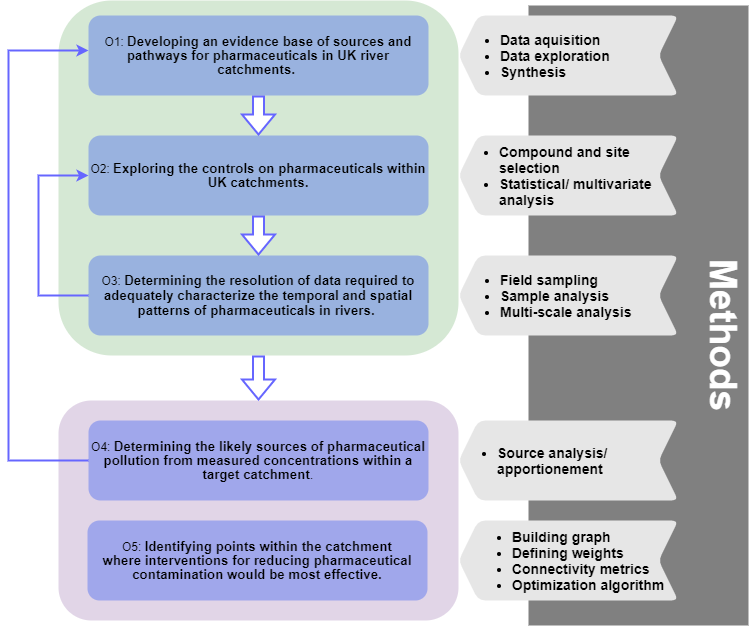
\includegraphics[height=10cm]{fig_workflow.png}
    \caption{Methods flow chart.}
    \label{fig_workflow}
\end{figure}

\subsection{Existing data}
\subsubsection{Data sources}
The main data set used for Objectives 1, 2, and 3 is the WIMS dataset, provided by the Environment Agency (EA) under a conditional license. The data is compiled using chemical analysis results for the Northeast and Yorkshire region in the UK, between 2005 and 2020, extracted from the Agency’s WIMS Water Quality Database. The dataset contains gas chromatography mass spectrometry (GC-MS) and liquid chromatography mass spectrometry (LC-MS) scan results for a total of 6738 samples collected at 610 sampling locations grouped within 73 river catchments. The vast majority of samples were taken from surface waters, but other sources include groundwater, sewage and trade discharge. The scans only provide positive results (meaning that where a chemical is not detected, there is no record of that chemical in the database), and as technological advancements have allowed more substances to be detected, the lack of a record for a specific compound does not imply a negative result. Furthermore, in recent years, LC has been used on an increasing proportion of screens, and is considered to provide a higher level of accuracy compared to GC (Figure \ref{fig_hist_and_maps}). The dataset contains records of 3084 unique analytes, of which 107 are pharmaceutical compounds.

\begin{figure}
    \centering
    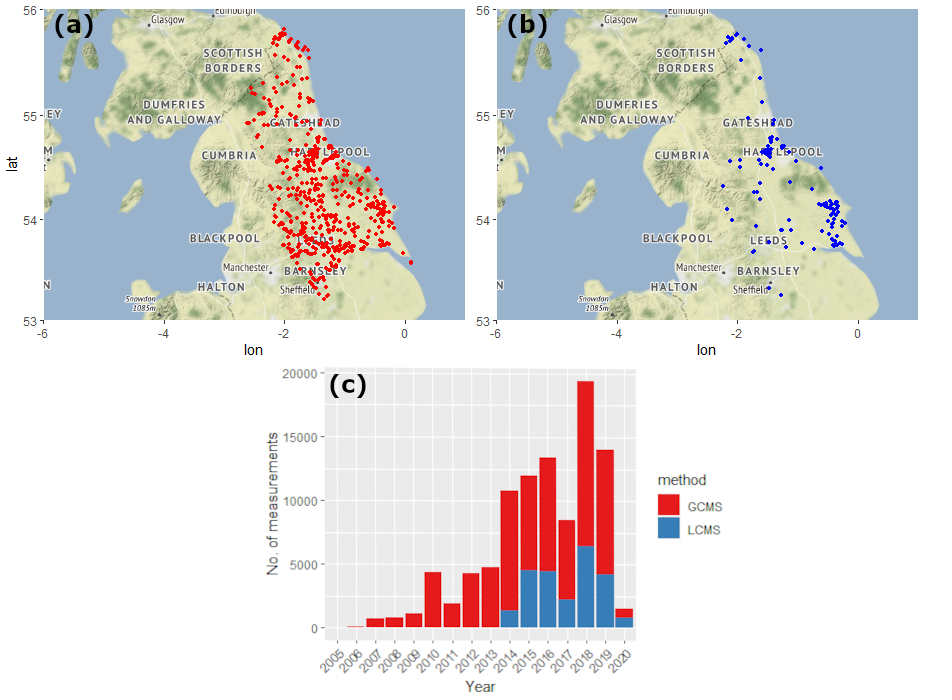
\includegraphics[height=10cm]{fig_WIMS_by_method.png}
    \caption{(top) Sampling sites for the WIMS data set, (bottom) number of measurements performed each year, grouped by the analytical technique used.}
    \label{fig_hist_and_maps}
\end{figure}

A second dataset  has been obtained from the open access Chemicals Investigation Program (CIP) online database. The project was undertaken by UK Water Industry Research (UKWIR) in order to aid the UK water industry in meeting the standards put forward by the WFD \citep{Comber2018ActiveConcern}. Building on a previous programme (CIP1, 2010-2014), the current phase (CIP2, 2015-2020) examines 74 substances of interest, including 19 pharmaceutical compounds and 4 metabolites, measured using variants of High Performance Liquid Chromatograph–Mass Spectrometry (HPLC-MS) or GC–MS  \citep{Comber2018ActiveConcern}. Samples were collected at over 600 WWTPs (Figure \ref{fig_cip_locations}a) selected based on an assessment of risk of high concentrations for the substances of interest in receiving waters due to low dilution rates \citep{UKWIR2017THEFINDINGS}. WWTPs were sampled for both influent and effluent, as well as receiving water sample points upstream and downstream of the corresponding discharge point. However, samples were only analyzed for pharmaceutical compounds at 45 of the WWTPs (Figure \ref{fig_cip_locations}b). The timeframe for the sampling is a two-year period between 2015-2017 with the sampling frequency differing for effluents and influents (20 sampling occasions) as opposed to river samples (36 occasions) \citep{UKWIR2019SUBSCRIBEPORTAL}.

\begin{figure}
    \centering
    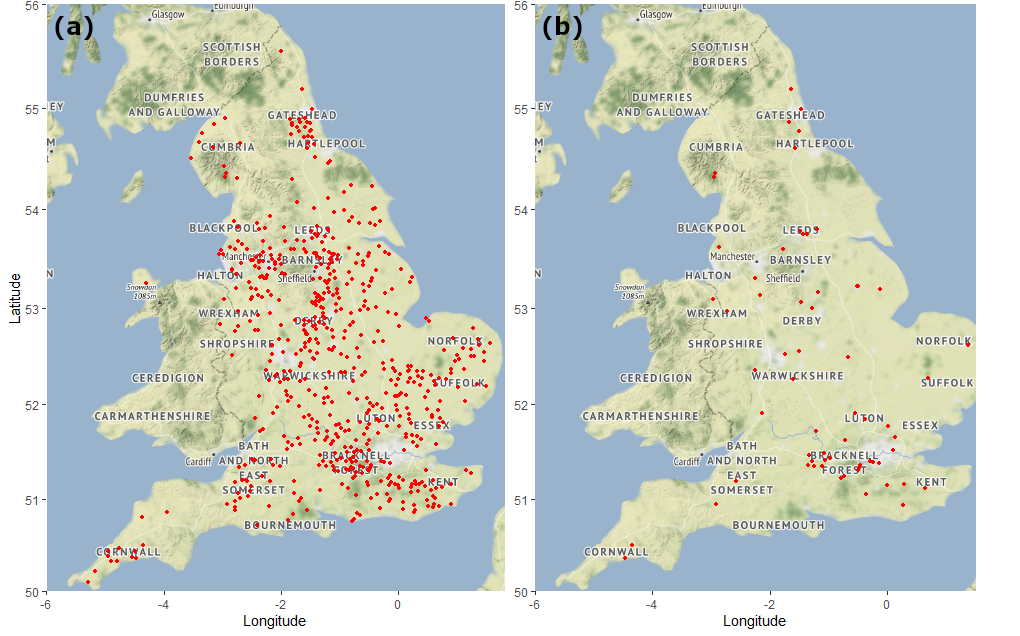
\includegraphics[height=10cm]{fig_CIP_locations.png}
    \caption{Sampling locations for the CIP dataset (a) all locations and (b) sites where data 
on pharmaceutical compounds is available.}
    \label{fig_cip_locations}
\end{figure}

The CIP dataset contains samples taken from a pool of sampling sites that while distinct, share a number of common sites with the WIMS dataset, and will be used to complement the latter, as illustrated in  of the following section. The WIMS and CIP databases have 11 pharmaceutical compounds in common (see Table \ref{table_compound_choice}). 

Additional data sources are summarized in  Table \ref{table_data_sources}. These data will be used to explore reasons for the spatial and temporal trends observed in the field data. The data will also be drawn upon in the research to address objectives 4 and 5.

\begin{table}
    \centering
    
\includegraphics[height=5cm]{logo.png}
    \caption{Additional data sources.}
    \label{table_data_source}
\end{table}

\subsubsection{Site selection}

At the current stage, preliminary analysis has been conducted in order to exemplify the methodology on two catchments selected for reasons of data abundance – the Ouse and Aire catchments (Figure \ref{fig_catchment_map}) and most measurements (6843 pharmaceutical concentration determinations for Ouse and 1188 for Aire, while Tees also ranks high with 1480) in the WIMS database. There is some overlap between the spatial distribution of sampling sites for WIMS and CIP within these two catchments, making the choice also suitable in terms of aggregating the two data sources (Figure \ref{fig_WIMS_locations}).


\begin{figure}
    \centering
    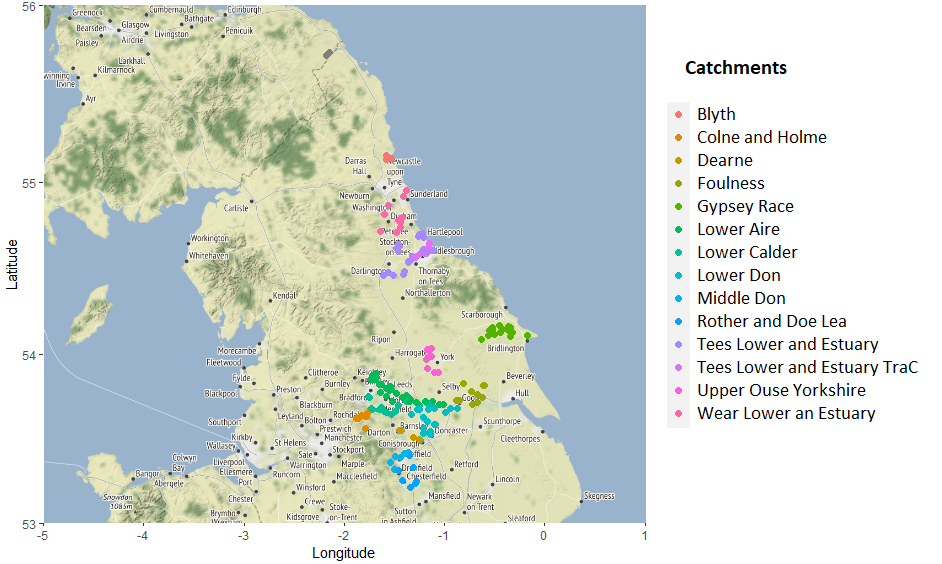
\includegraphics[height=10cm]{fig_catchments_map.png}
    \caption{Sampling sites in the WIMS dataset, for each catchment (only the 12 catchments with most locations represented).}
    \label{fig_WIMS_locations}
\end{figure}

Several additional factors (Table \ref{table_catchment_choice}) will play a part in the next step in determining the catchment/catchments that will be the subject of the analysis for O2 and the location of the field sampling for O3.

\begin{table}
    \centering
    
\includegraphics[height=5cm]{logo.png}
    \caption{Decisional factors considered in the process of selecting the specific catchment/catchments to be studied).}
    \label{table_catchment_choice}
\end{table}


\begin{figure}
    \centering
    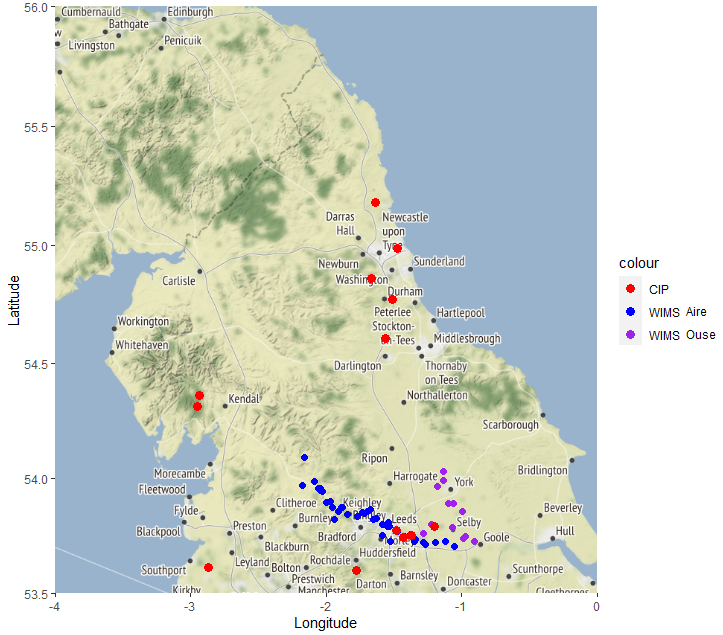
\includegraphics[height=10cm]{fig_catchments_wims_cip.png}
    \caption{Comparing sampling locations between (red) CIP sampling sites (where pharmaceutical concentrations are available) and (blue, purple)) WIMS sampling sites in the Aire and Ouse catchments.}
    \label{fig_catchment_map}
\end{figure}

\subsubsection{Pharmaceutical compound selection}
In order to limit computational complexity and laboratory analysis costs, the analysis will focus on a restricted set of pharmaceutical compounds. The choice of compounds will be based on a number of factors outlined in Table \ref{table_compound_choice}. Considering that the first two objectives deal exclusively with existing data sets, it is only natural to first consider which compounds are represented in these data sets with sufficient temporal and spatial frequency to provide data points. Across the entire WIMS dataset, Caffeine, Carbamazepine and Gabapentin account for most detections.


\begin{figure}
    \centering
    
\includegraphics[height=5cm]{logo.png}
    \caption{Decisional factors considered in the process of selecting the specific compounds (or compound classes) to be analyzed in the samples collected}
    \label{table_compound_choice}
\end{figure}

\subsection{Field data collection}
\subsubsection{Sample collection}
\subsubsubsection{Sampling method}
Given uncertainties related to the ability to conduct field work in the foreseeable future as well as several decisions relating to compound and catchment selection being depended on the ongoing analysis (O1 an O2), planning the field work remains at an early stage. Careful consideration will be paid to formulating a field sampling strategy, considering that the quality of data obtained is highly dependent on reducing sampling errors and biases \citep{Ort2010SamplingReview}. Across the literature on pharmaceuticals in the environment, there is no standard procedure across all studies, with some opting for a one-time grab sampling, while others use 24h composites \citep{Verlicchi2012OccurrenceReview}. Furthermore, monitoring schemes rarely provide enough repeated samplings to cover short-term or seasonal variation \citep{Ort2010SamplingReview} and the number of sampling sites is too limited and often biased towards  hot spots such as WWTPs or convenient sampling locations such as gauging stations \citep{ausderBeek2016PharmaceuticalsPerspectives}. 

In the case of CIP, grab sampling was preferred due to concerns over analyte stability and as a means of illustrating variation within compliance measurements which themselves usually are performed using grab samples \citep{Gardner2012TheEffluents}. However, in order to capture short-term variation, a flow-proportional or volume -proportional composite sample may be required, unless a pre-experiment can be conducted to show that diurnal variation is not significant \citep{Ort2010SamplingReview}. Regarding river samples, one mid-stream sample is usually considered representative of the concentration for the cross-section although several samples at different vertical profiles have also been proposed \citep{Comoretto2005ComparingRiver}.

In order to develop the fieldwork strategy for this proposed research, a preliminary grab sampling campaign is planned.The primary aim of this campaign would be to inform sampling location choices - based on presence-absence results for the target compounds at an inital selection of sites - as well as to assess diurnal and daily variation in pharmaceutical concentrations in order to determine an appropriate temporal frequency for sampling in a later campaign. This 

\subsubsubsection{Sample stability}
An important factor to consider in developing the sampling protocol is sample stability. Pharmaceutical compounds (as well as their metabolites and transformation products) vary considerably in terms of how long samples may be kept before concentrations are significantly decreased \citep{Caban2015AnalyticalProspects} or whether stabilizing agents or processes such as chilling can be applied to increase this time. As such, the choice of pharmaceutical compounds (see Table \ref{table_compound_choice}) will be influenced by existing literature on the stability of specific compounds. In the case of pharmaceuticals included in the CIP dataset, the sampling protocol can be inspired by that of the CIP program which was informed by a precursory study \citep{Gardner2012SampleWastewater} verifying that sample concentrations would not change by more than 25\%. Accordingly, the protocol requires that pharmaceuticals be kept in glass vessels, chilled to 3°-5°C and analyzed within 5 days, with the exception of the three steroids which may be preserved for 14 days, but require amber glass bottles as well as an in-field pre-treatment step (filtration to 1µm using a glass fiber filter) and preservation with 30\% hydrochloric acid and copper nitrate \citep{UKWIR2015DraftGuidance}.

Depending on the choice of compounds and whether there will be restrictions that limit field activities during the initial phase of the proposed research, a pilot study establishing stability of the chosen compounds can be undertaken, particularly for compounds not covered by CIP and for which existing stability studies are not found in the literature.

\subsubsection{Analytical methods}
Water samples are commonly screened for target compounds using LC-MS or GC–MS. As pharmaceuticals are typically highly polar, they are less suited for GC-MS, but can be made available to this procedure through derivatization \citep{Postigo2014TransformationTreatment}, which is the process of converting less volatile analytes to substances that can be analyzed in a gaseous state through chemical reaction with one or more derivatizing reagents. Advances in mass spectrometry techniques have enabled higher resolution (such as using time-of-flight (TOF), quadrupole TOF, or Orbitrap mass spectrometers) and with it, the identification of unknown transformation products. These identified structures can then be confirmed using nuclear magnetic resonance (NMR). 

Following sample collection, the samples will be analyzed in the Analytical Laboratory of the Geography Department of Durham University. The laboratory is equipped with several analytical devices suited for measuring pharmaceutical concentrations, including an Inductively Coupled Plasma - Mass Spectrometer (ICP-MS), several GC-MS units as well as an Ultra-High Performance Liquid Chromatograph – Mass Spectrometer (UPLC-MS/MS). The analytical protocol may be informed by Method 1694 (Epa, 2007), which has been recommended by the European Pharmaceuticals Agency (EPA) as the standard for the determination of 70 pharmaceuticals \citep{Caban2015AnalyticalProspects}. However, specific analytical procedures may be determined based on the sampled matrix as well as the chosen compounds of interest, which would require specific chromatography columns or derivatization agents.

\subsection{Data analysis}
\subsubsection{Data modeling and statistical methods}
In order to assess the contribution of different factors in determining concentrations of pharmaceutical compounds in environmental samples as part of O2, statistical analysis will be performed on the compiled datasets using the R language and RStudio \citep{R.Development.CoreTeam2010R:Computing.}. Possible analyses in order to describe patterns explained by the predictor factors under consideration may include multiple regression or principle component analysis as illustrated by \citet{Giglioli2020SourceNaples} in a study of contaminant concentrations in a marine environment.

\subsubsection{Graph theory}
The graph theory approach will be developed over the course of the PhD and informed by the understanding of pharmaceutical dynamics in the target catchments gained in the previous stages as well as by the advanced training in Graph Theory (item 1.7. in Table \ref{fig_gantt}). 

A first step will be to develop a conceptual representation of the catchment as a graph. This will depend on the framing of the management problem that needs to be addressed, which will itself be refined as the exploration of the data and catchment-specific dynamics is undertaken. Several approaches that exist in the literature may be modified to suit this purpose (Figure \ref{fig_graph_eros}), and a means of assigning weights to the edges of the graph (similar to that detailed in Figure \ref{fig_graph_schick}) may be developed to take into account pharmaceutical transmission rates or removal costs for example.

\begin{figure}[h]
    \centering
    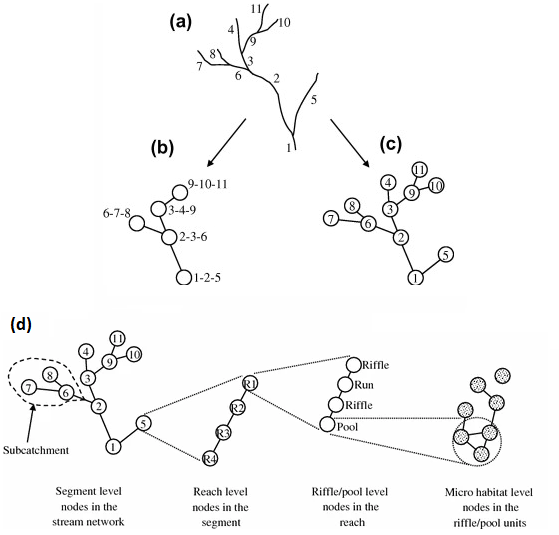
\includegraphics[height=10cm]{fig_graph_eros.png}
    \caption{Two simple approaches to representing a river network (a) by using confluences as either (b) nodes or (c) links between river segments  – figure taken from \citet{Eros2011NetworkApproach},
 and (d) representations of the same network at multiple scales - taken from \citet{Eros2012CharacterizingGraphs}. 
}
    \label{fig_graph_eros}
\end{figure}

Among the possible applications of graph theory in the proposed research, the concepts of critical nodes and flows seem to have the most potential to shed light on effective intervention points and strategies. Critical node identification, defined as the problem of pinpointing a subset of nodes whose removal maximizes network fragmentation \citep{Lalou2018TheSurvey,Sarker2019CriticalNetworks}, may be performed and assessed to determine whether the critical nodes would be suitable as priority intervention points. Likewise, a modified approach based on the minimum cut-max flow theorem \citep{Anderson2020ComplexApplications} could be employed to identify a set of edges in the graph that, when impeded, would most reduce transmission of pharmaceuticals through the system.

In terms of connectivity indices, there is much discussion in the literature about the relative benefits and drawbacks of the many different available options \citep{Ali2010ShoppingCatchment,Saura2007AStudy}, and these resources will inform the choice of metric. The chosen indices may be computed for the current state of the system as well as for proposed mitigating scenarios and the changes in value interpret to designate favorable measures. Lastly, the temporal dynamics of the connectivity of the system may be investigated using multiplex network \citep{Pearson2020SedimentPathways}. 
There are dedicated connectivity packages in R and python, as well as MATLAB \citep{Rubinov2010ComplexInterpretations}, which will be assessed in order to determine the more suitable option for this particular application.

\subsubsection{Source analysis}
 \label{source_analysis}
Having access to pharmaceutical compound signal data at various points in a catchment raises the question of whether this data can help trace back the contaminants to a likely source. A possible means of addressing this problem may be derived from a similar application in the field of neuroscience, particularly magneto-encephalography (MEG) signal analysis \citep{Taylor1999MathematicalExpansions}.  Also known as the inverse problem in signal analysis, this framework tackles the problem of identifying contributing sources based on a measured final signal, and has been applied in the literature in the context of instantaneous river pollution \citep{Han2014InverseAccuracy} and using pollutant transport models for groundwater pollution source identification \citep{Gurarslan2015SolvingAlgorithm,Jamshidi2020SolvingOptimization}.

An i-CONN training course on ‘Advanced Matlab for pre-processing, visualization and controlling toolboxes and packages in pipelines’ (item 1.6. in the Gantt Chart in Table \ref{fig_gantt}) provided by the AAI Scientific Cultural Services will be the basis to explore the viability of performing source analysis in the context of the current research. This interdisciplinary course based in neuroscience is ongoing and addresses the field-specific methods of solving the inverse problem. 

\clearpage
\section{Initial results}
An initial exploration of the WIMS data set has revealed a number of preliminary results that will be further analyzed in order to meet objectives 1 and 2. The CIP data set has not yet been explored as precise sampling location data is in the process of being delivered.

The dataset was initially subjected to a cleansing, notably eliminating erroneous locations and database entries that could not be provided with a unique compound code (the identifier used in the database is the CAS number, a unique identifier assigned in a registry for chemical substances by the Chemical Abstracts Service), many of which containing only comments in the analyte name field.

A first exploration of the temporal distribution of sampling across the WIMS dataset revealed that sampling effort was unevenly distributed, favoring spring and fall months, and sampling times were unsurprisingly biased towards working hours (Figure \ref{fig_general_hist}).

\begin{figure}[h]
    \centering
    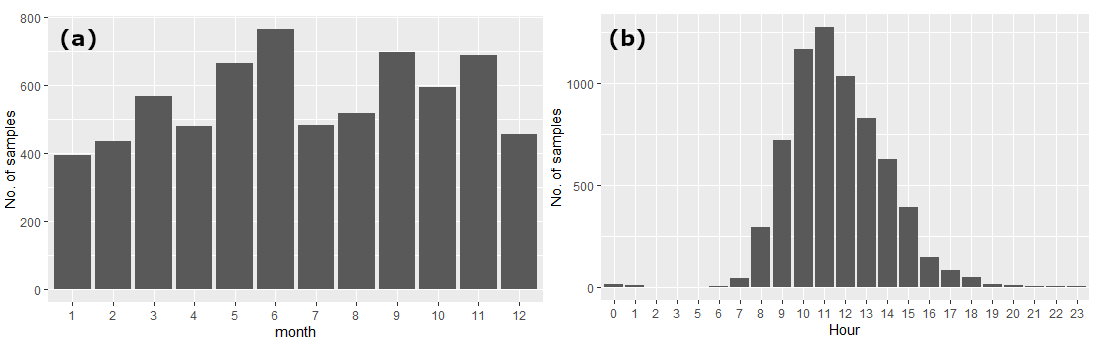
\includegraphics[height=5cm]{fig_hist.png}
    \caption{General temporal distribution of samples taken within the WIMS dataset: histogram of sample distribution according to (a) month of the year and (b) hour of the day.}
    \label{fig_general_hist}
\end{figure}

Subsequently, in order to examine how spatial patterns of pharmaceutical concentrations may be captured by the WIMS dataset, the antiepileptic compound carbamazepine was chosen as an example (Figure \ref{fig_carbamazepine_map}). Carbamazepine is particularly useful as a stand in in this illustrative example as it has been proposed as a suitable marker for anthropogenic influences in the aquatic environment due to its persistence and frequent occurrence in freshwater samples \citep{Clara2004CarbamazepineInfiltration}.

\begin{figure}[h]
    \centering
    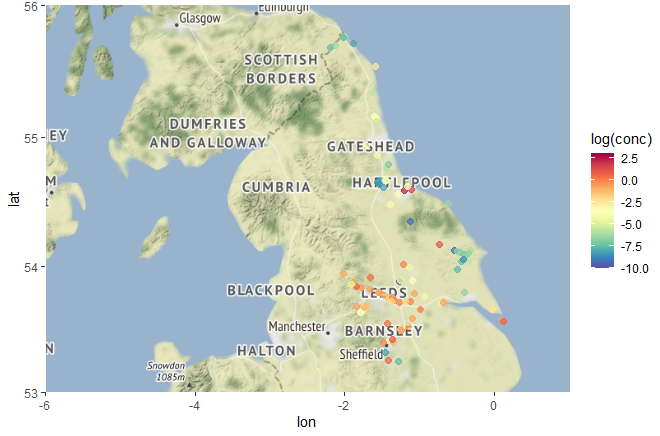
\includegraphics[height=9cm]{fig_carbamazepine_map.png}
    \caption{Map of average carbamazepine concentrations over the whole monitoring period (log scale).}
    \label{fig_carbamazepine_map}
\end{figure}

The next step was to explore long-term trends in concentration of specific compounds. In order to avoid any bias introduced by the uneven sampling across the set of sampling sites, some of which were sampled regularly and some on just one occasion for example, the long-term trends were analyzed at specific sampling locations as opposed to over the entire study area. The sites were chosen from the two catchments which had the highest number of records in the WIMS database – the Ouse and Aire catchments- and of those, the sampling site (Figure \ref{fig_ouse_site_map}) and compounds (Gabapentin, Diclofenac and Lidocaine) with the most samples were selected. 

\begin{figure}[h]
    \centering
    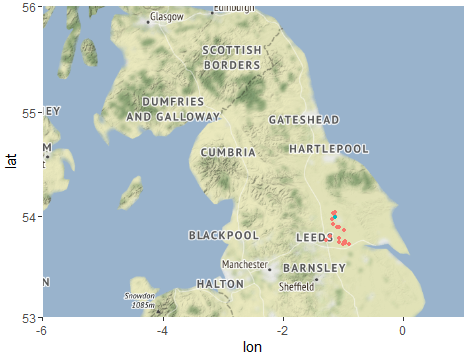
\includegraphics[height=10cm]{fig_ouse_site_map.png}
    \caption{Map of WIMS sampling locations in the Ouse Catchment, highlighting the Nether Poppleton (Skelton) sampling location (blue) used in the following analyses.}
    \label{fig_ouse_site_map}
\end{figure}

Furhermore, although initial results comparing LC-MS and GC-MS results for sites and compounds where both methods were used suggest that the method used does not introduce any bias (Figure \ref{fig_lc_gc_boxplot}), for the purpose of this initial exploration, only LC-MS data is used, as it is considered to be more accurate \citep{Stout2009ABenzoylecgonine}.

\begin{figure}[h]
    \centering
    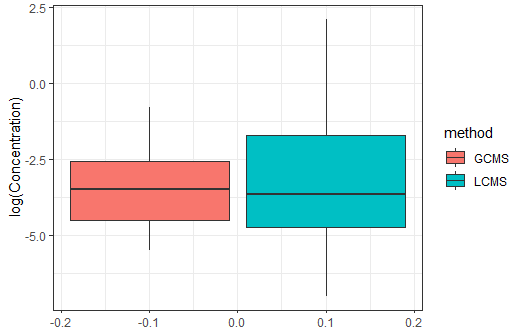
\includegraphics[height=7cm]{fig_boxplots.png}
    \caption{Concentration boxplots for each sampling site and Pharmaceutical compound combination
 where both methods (GC-MS and LC-MS) were used.}
    \label{fig_lc_gc_boxplot}
\end{figure}

Although these time series suggest a decrease over the last five years for the chosen compounds, these preliminary results should be viewed with caution as gaps in the time series may skew the results, particularly seeing as there is a strong seasonal variation, as illustrated by Figure \ref{fig_ouse_site_time_series} and Figure \ref{fig_ouse_site_seasonality}. The exploratory analysis will be continued in order to verify whether there is indeed a downward trend or if it is an artifact of the sampling gaps.

\begin{figure}[h]
    \centering
    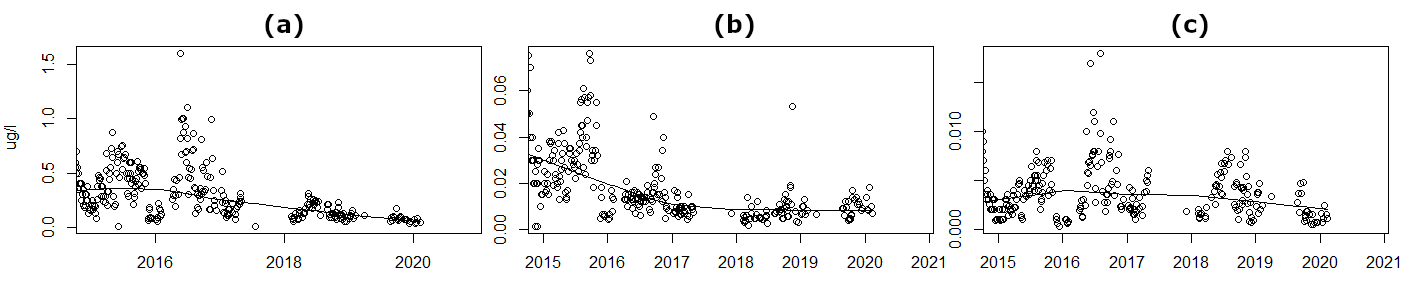
\includegraphics[height=3.5cm]{fig_time_series.png}
    \caption{Concentration time series for the interval 2015-2020 at Nether Poppleton (Skelton) sampling site (Ouse catchment) 
for (a) Gabapentin, (b) Diclofenac, (c) Lidocaine.}
    \label{fig_ouse_site_time_series}
\end{figure}


\begin{figure}[h]
    \centering
    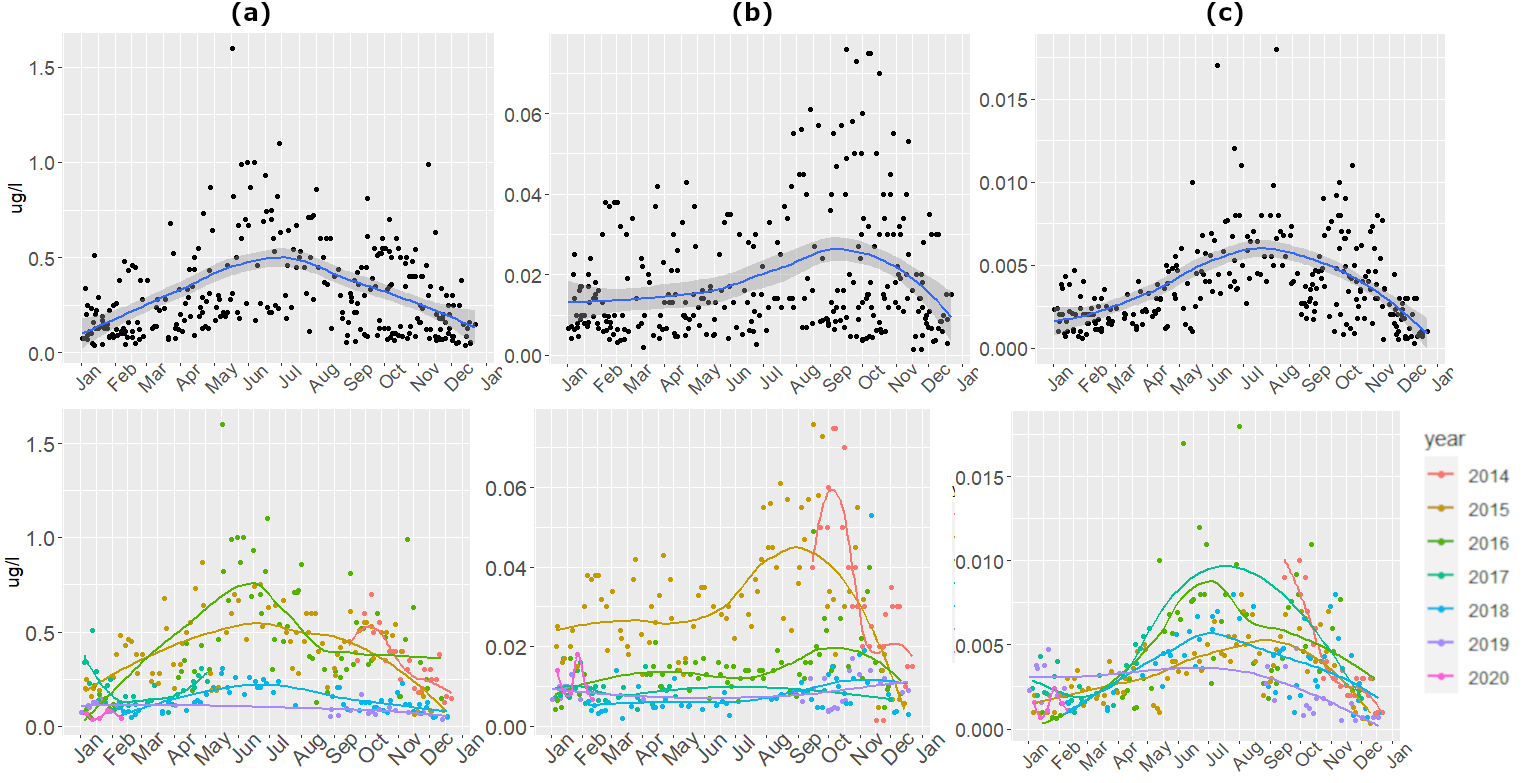
\includegraphics[height=8cm]{fig_seasonality.png}
    \caption{Seasonality of LC concentrations at Nether Poppleton (Skelton) sampling site (Ouse catchment) for (a) Gabapentin, (b) Diclofenac, (c) Lidocaine. For each: (top) concentrations plotted by date across the years 2015-2020 with trend line and confidence interval; (bottom) seasonal trendline grouped by year.}
    \label{fig_ouse_site_seasonality}
\end{figure}

\clearpage
\section{Conclusions}

\subsection{Expected outcomes}
The first outcome is expected to be an integrated database of pharmaceutical occurrence data for UK catchments, accompanied by a comprehensive description of its scope, gaps and significance for the issue of pharmaceuticals in the environment. The analysis of this data corresponding to O2 will produce statistical models of pharmaceutical concentrations as a function of the chosen factors. This statistical analysis is expected to give an indication of the significance of these factors and their interactions. 

According to the plan set out in O3, a dataset of measured pharmaceutical concentrations will be compiled following the field sampling performed over a representative timeframe (ideally over the course of a year, but subject to modification). The samples will be collected at a chosen catchment/catchments at the highest spatial and temporal frequency allowed within practical constraints. Subsequently, a multiscale analysis comparing the representation of the catchment provided by the collected data to that permitted by the coarser resolution data (from O1) will produce an assessment of the scale and resolution required to capture pharmaceutical dynamics in river catchments.

The analysis planned for O4 is expected to offer a set of likely locations or types of significant sources of pharmaceutical contamination based on the existing and collected datasets. Using this enriched understanding of sources and pathways, the final proposed objective will provide a supporting tool for targeted management decision-making. This will take the form of a graph representation of the catchment system that is suitable for framing and resolving intervention optimization questions.

\subsection{Potential challenges}
Given continuing restrictions in the UK and uncertainty regarding the evolution of the pandemic, there may be difficulty in collecting new samples for the purpose of this research. However, the availability of existing datasets offers the possibility of accomplishing the objectives even in this scenario, with the exception of O3, which may be adapted to use subsets of the existing datasets with different temporal and spatial frequencies.

Secondly, the suitability of some of the proposed methods (corresponding to O4 and O5) will only be determined after undertaking advanced training in the respective fields over the course of the PhD program. Should these methods prove inadequate in this context, alternative methods to achieving the stated objectives will be investigated (for example, source apportionment \citep{Gasperi2010ContributionsSystems,Giglioli2020SourceNaples} as an alternative to source analysis).

\subsection{Timeline}
 A Gantt chart detailing the timeline of the necessary steps for undertaking the proposed research is presented in Table 5.
 
\begin{landscape}
\newgeometry{margin=0.5in}  
\begin{figure}
    \centering
    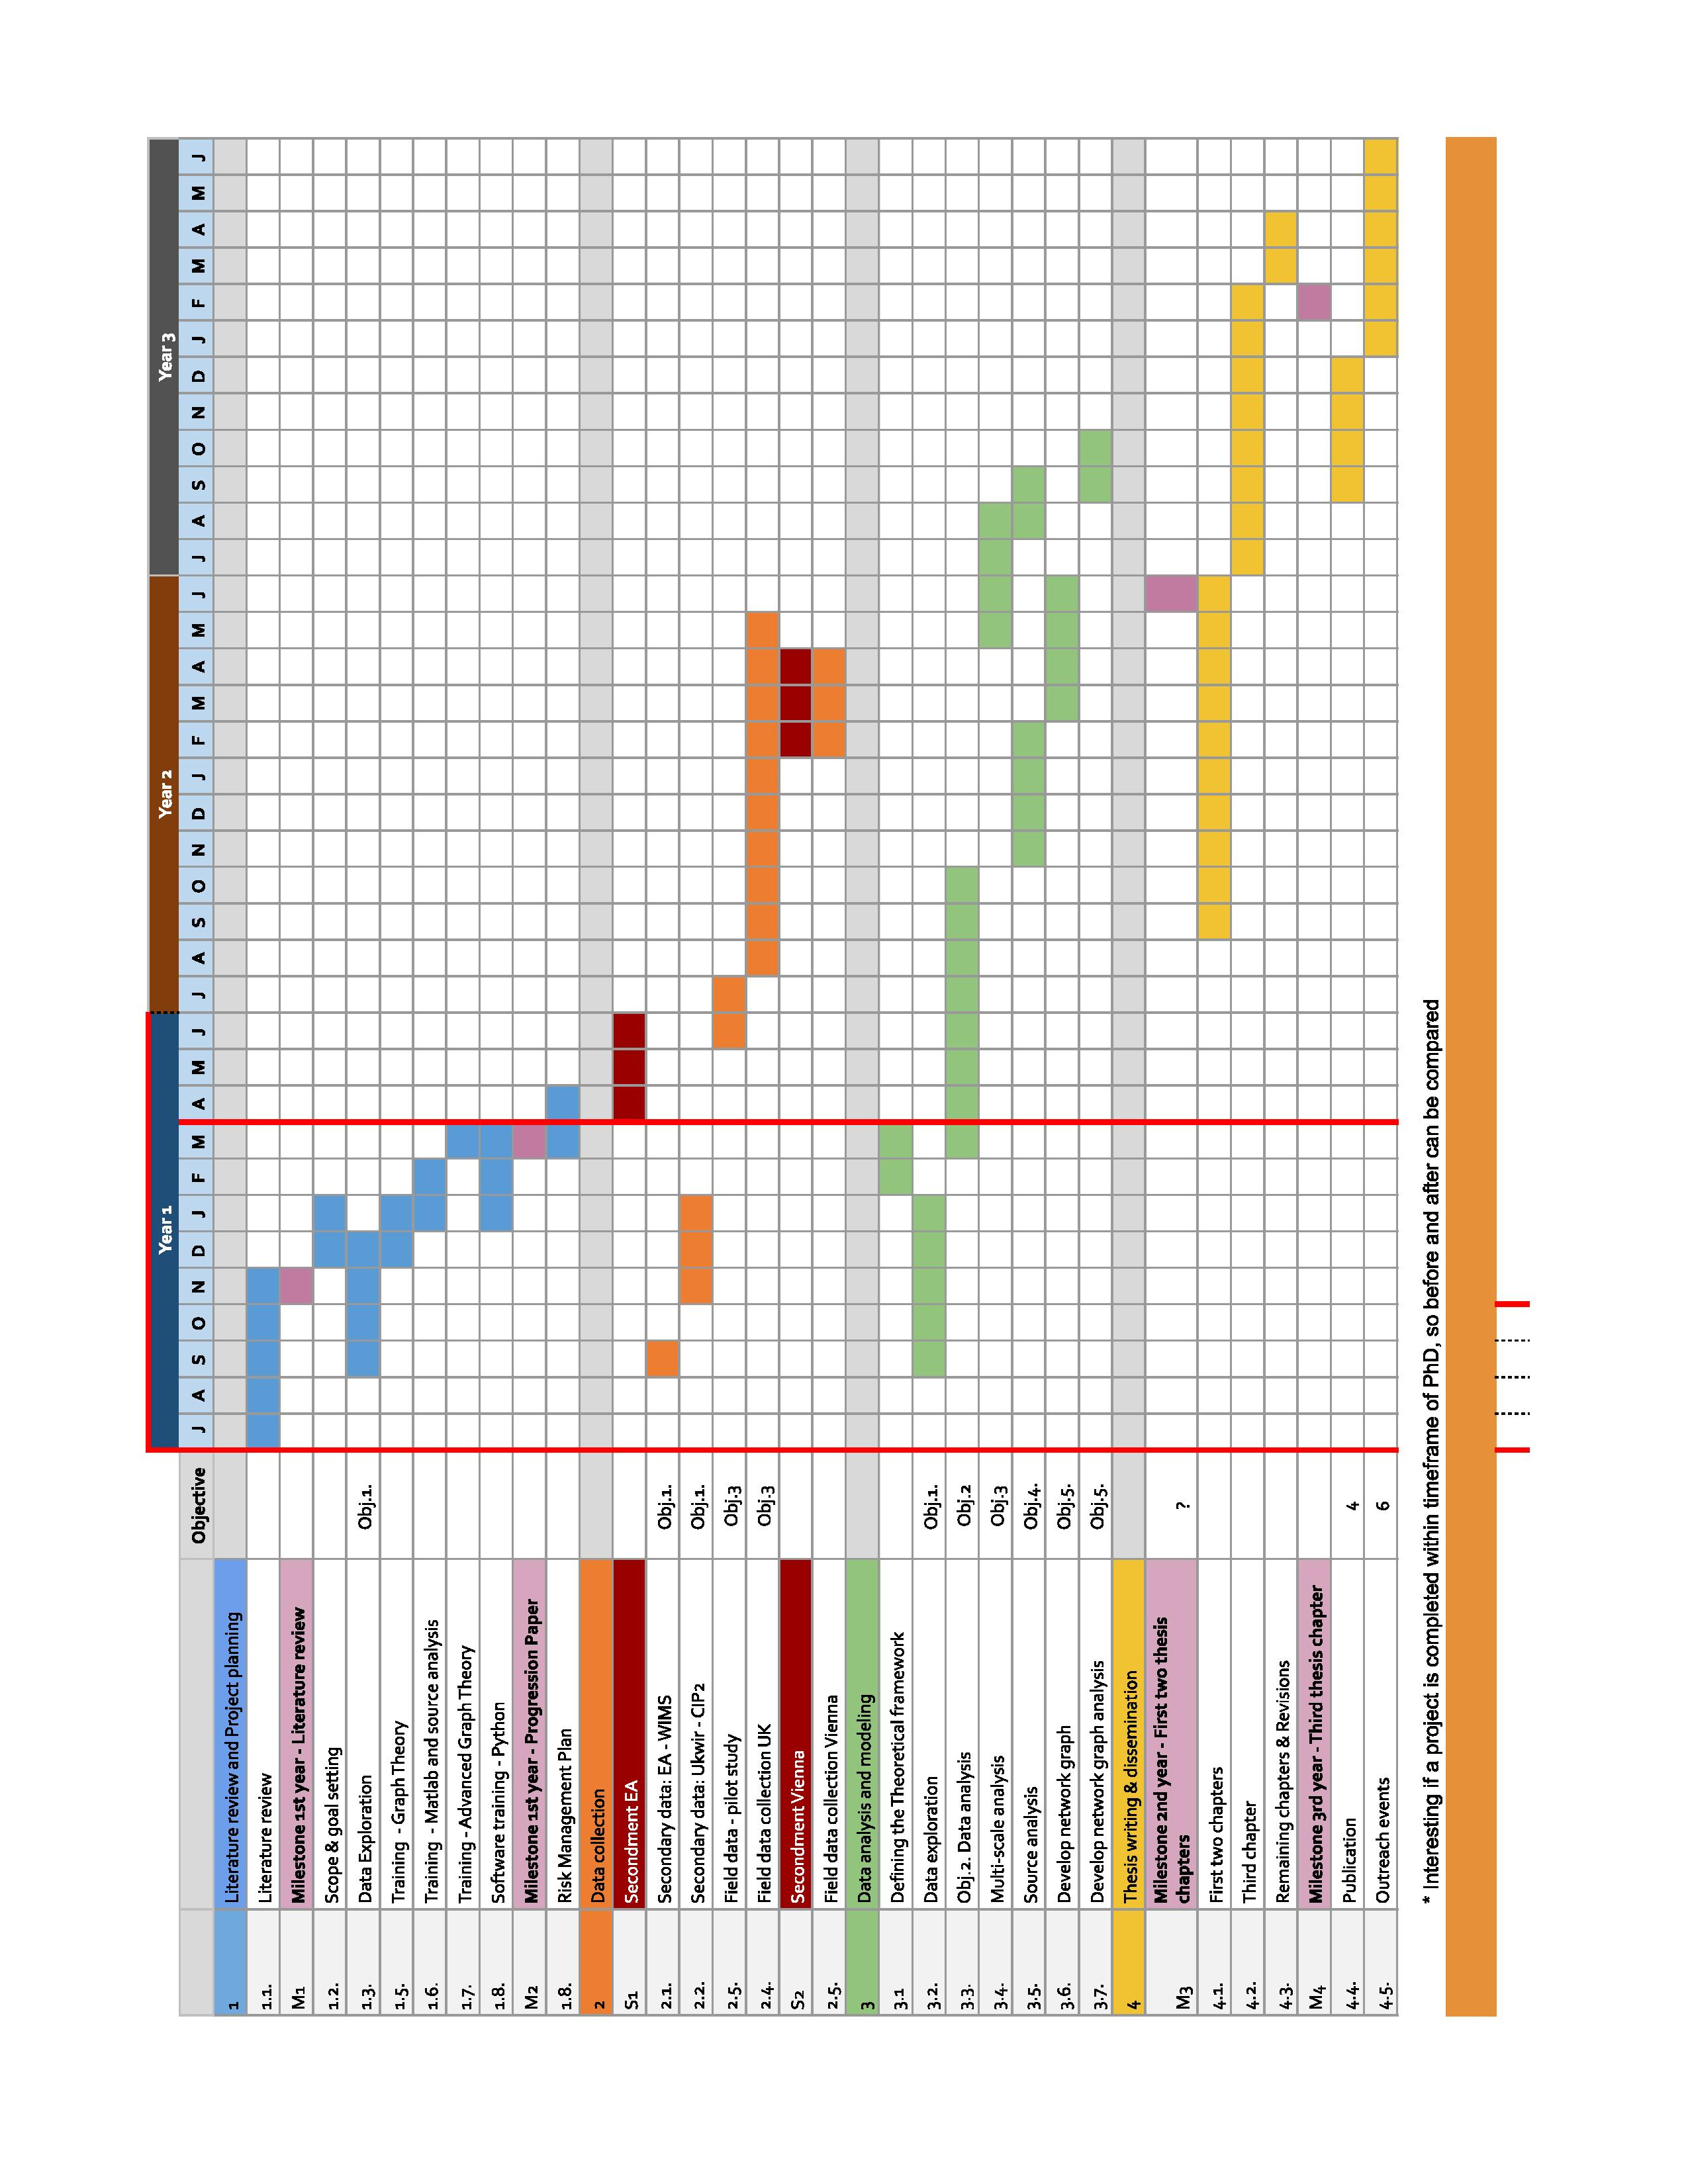
\includegraphics[angle=270,origin=c, height=10cm, trim=0 0 4.5cm 0, clip]{fig_gantt.jpg}
    \caption{Gantt Chart of the PhD project.\footnotemark }
    \label{fig_gantt}
\end{figure}
\footnotetext{The i-CONN project includes secondments with partner institutions, in this case, the BOKU university in Vienna. As of the editing of this document, activities to be conducted during the secondment remain to be determined. Two possibilities are (a) apply analyses and network-approached developed for UK catchments for a local catchment using either existing pharmaceutical data or field data collected during the secondment or in advance by collaborators at BOKU or (b) learning to use community composition analysis applied by ESR 8 for invertebrate macro-communities to investigate patterns in pharmaceutical mixtures}
\restoregeometry
\end{landscape}

%\printbibliography{references.bib} %with biblatex
\clearpage
%\bibliographystyle{agsm}
\bibliographystyle{elsarticle-harv}
\bibliography{references}

\clearpage
\section*{Appendices}
\subsection*{A1 – Planned resource form}
(postgraduate handbook 2020-2021, Apendix 1, p55)


Guidance: Using the table below, please briefly outline the main resources you plan to use for your research programme. Where relevant or known, please give an indication of timing, and for laboratory work, how many samples you anticipate analysing. At this early stage of your research you may not have finalised these details, and your plans are likely to evolve as your research progresses. Use this form as an initial scoping of what you may require, based on your Progression Paper proposal. You may wish to edit your form following your Progression Panel discussions, and return a revised version to the PGR office. All forms will be reviewed by the Director of Services and Chief Technician, who will contact you if they have any concerns. As your research programme develops, you are encouraged to discuss any changes to your resource needs with your supervisors, the Director of Services and/or the Chief Technician. 

A full list of Department Facilities will be made available via the department website in due course.. Note that the Department laboratories and technical staff look after a range of resources for both human and physical geography.



\end{document}
